

%Overskrift
\begin{center}
\Huge
Differentialregning
\end{center}
\section*{Differentialkvotienten}
\stepcounter{section}

Differentialregning går lidt løst sagt ud på at se på hvordan "pæne" funktioner ændrer sig lokalt. Vi vil kun ganske uformelt diskutere, hvad der menes med pæne funktioner. Vi vil starte med at betragte et eksempel.
\begin{exa}
Vi forestiller os, at vi kører i en bil, og vi er interesserede i hvor stærkt, vi kører på et tidspunkt $t$. Lad os sige, at vi fra tidspunkt $t$ til tidspunkt $t+5$ måler, at vi er kørt $200m$. Så ved vi, at vi i gennemsnit har kørt med en hastighed på
\begin{align*}
\frac{200m}{5s} = 40\frac{m}{s},
\end{align*} 
men vi ved fortsat ikke, hvor stærkt vi kørte nøjagtigt ved tid $t$. Vi måler derfor, at vi til tidspunkt $t+2$ har kørt $70m$. Vi ved derfor, at vi fra tid $t$ til tid $t+2$ har kørt med en hastighed på 
\begin{align*}
\frac{70m}{2s} = 35\frac{m}{s},
\end{align*}
og vi kommer en smule nærmere den korrekte hastighed til tid $t$. Den korrekte hastighed må derfor blive tilnærmet mere og mere jo mindre tidsinterval, vi måler hen over bliver. 
\end{exa}
Inspireret af dette eksempel, vil vi definere den såkaldte differentialkvotient, der fortæller noget om den øjeblikkelige tilvækst af en funktion. 
Betragt funktionen på Fig. \ref{fig:sek1}
\begin{figure}[H]
\centering
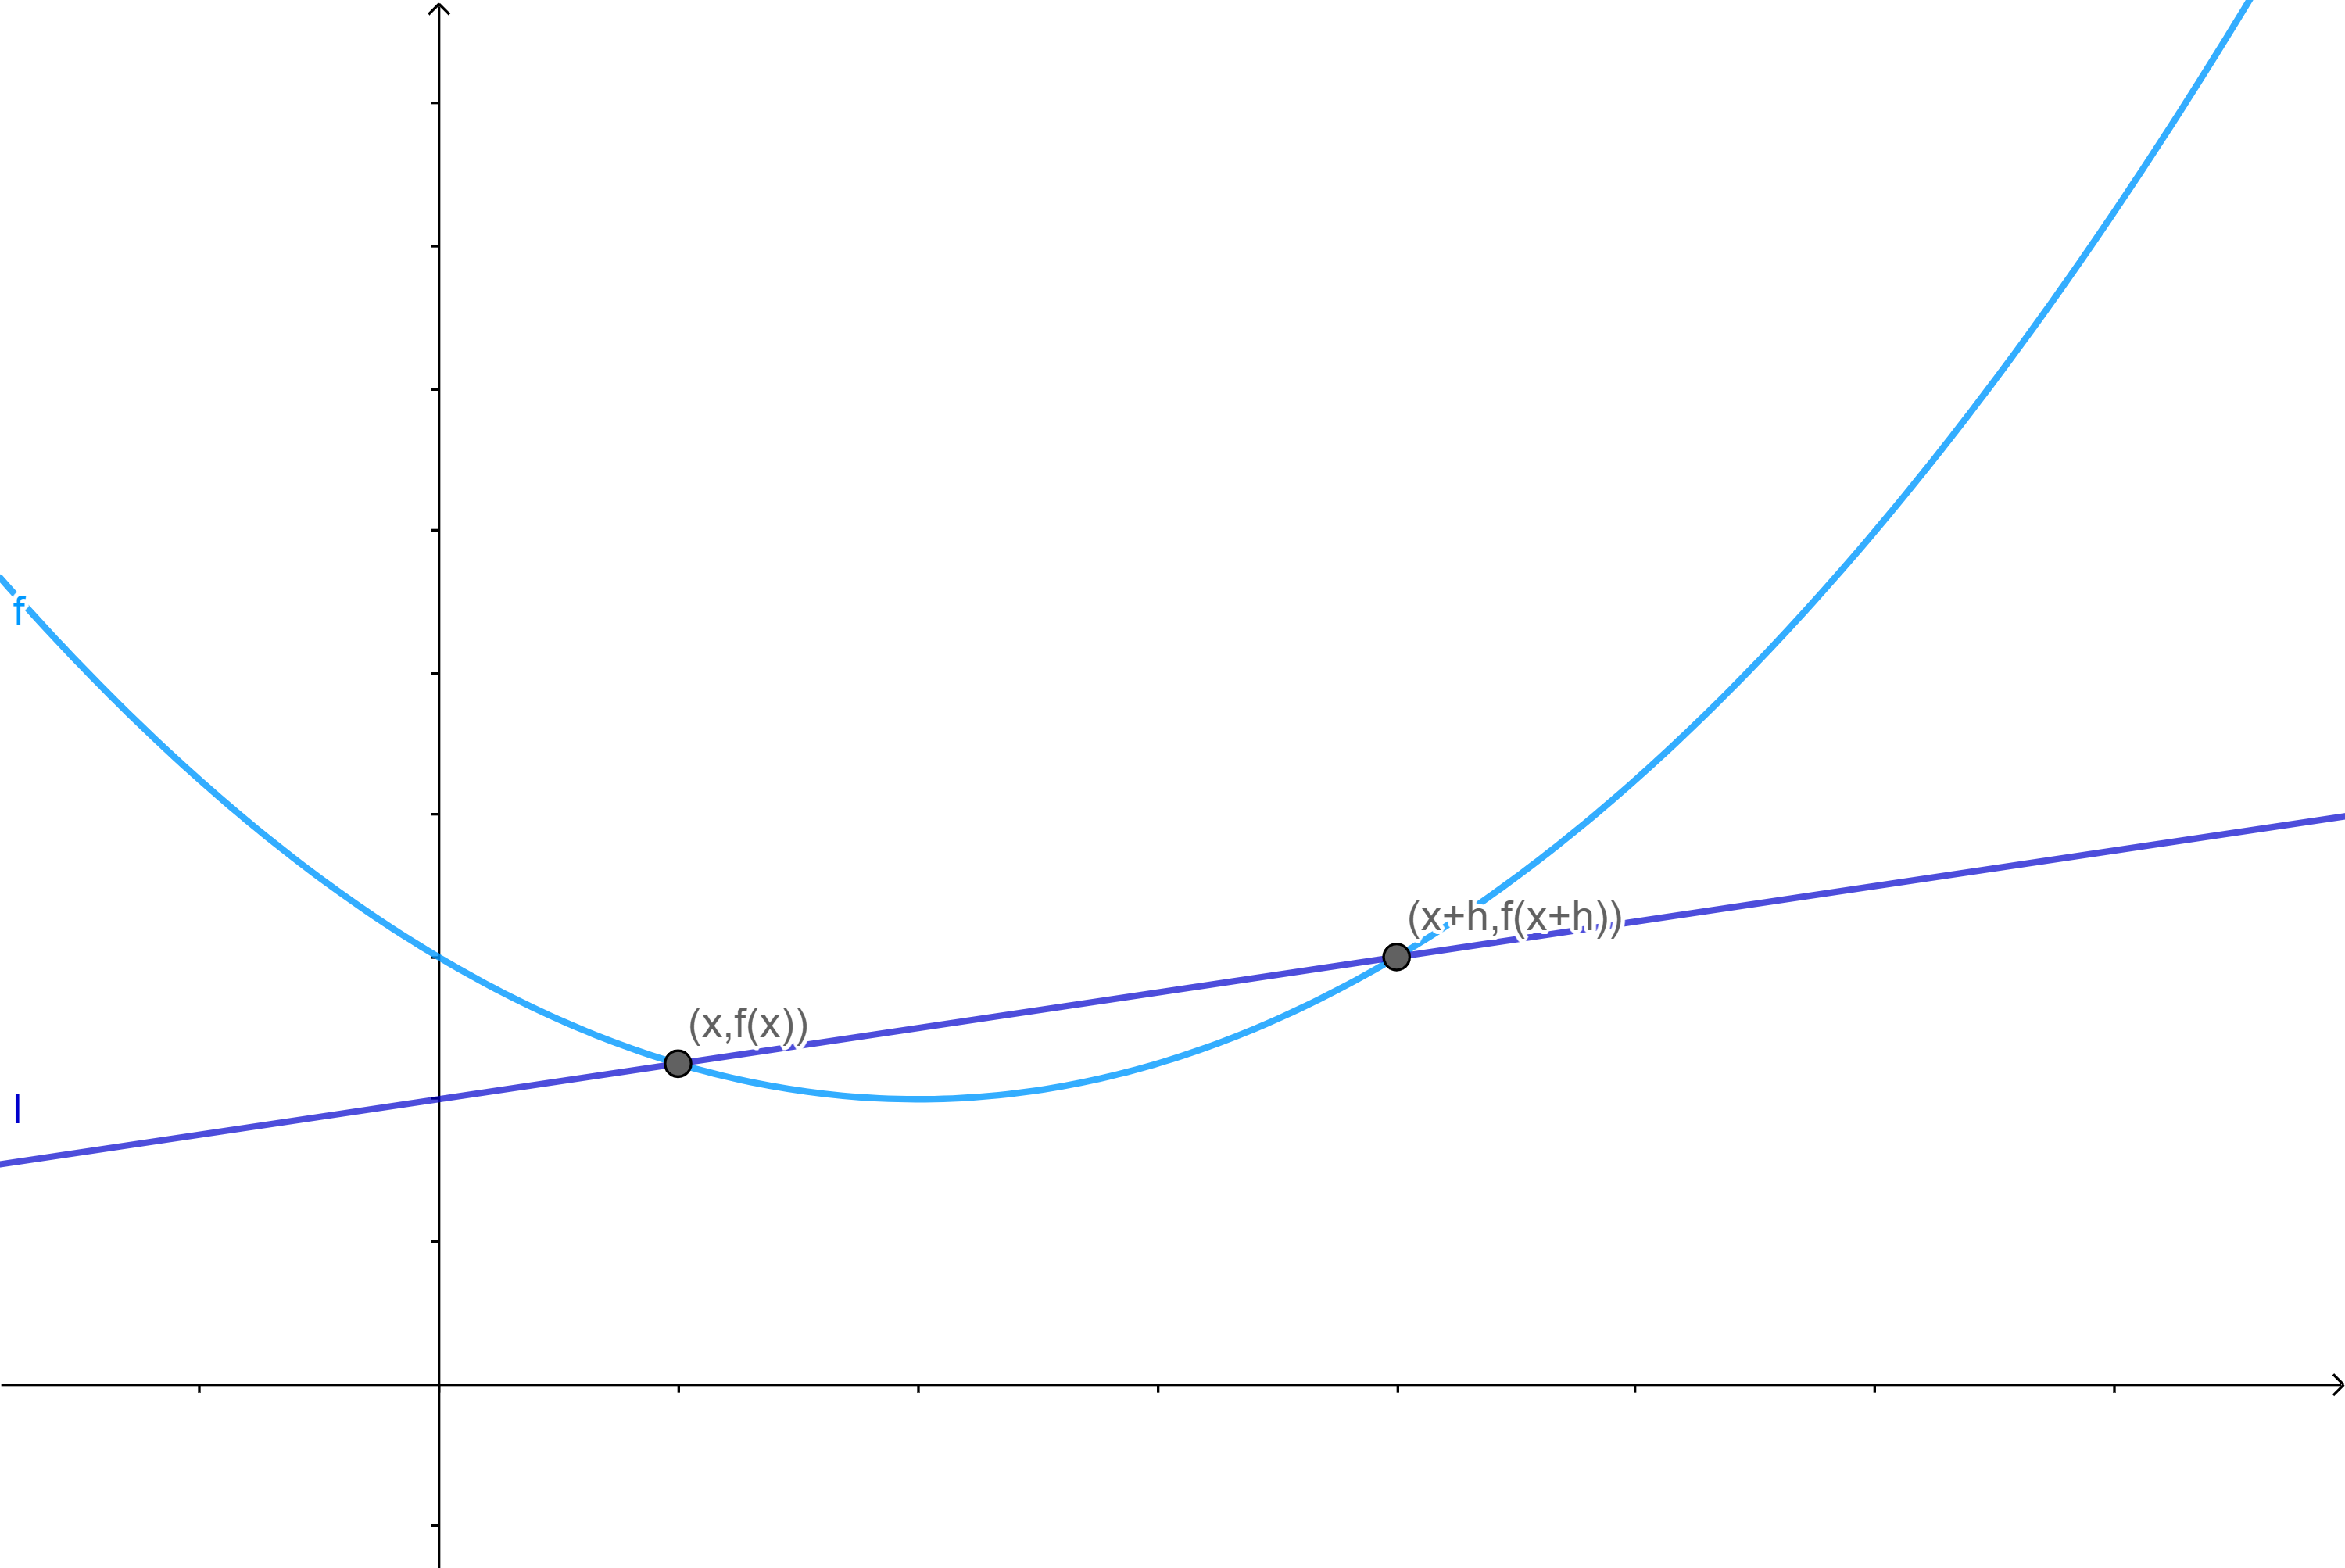
\includegraphics[width = 12cm]{Billeder/sekant1.png}
\caption{Funktion med sekant gennem punkterne $(x,f(x))$ og $(x+h,f(x+h))$.}
\label{fig:sek1}
\end{figure}
Lader vi $h$ blive mindre, så vil sekanten gennem punkterne $(x,f(x))$ og $(x+h,f(x+h))$ komme tættere og tættere på at være tangent til funktionen $f$ i punktet $(x,f(x))$, som vi ser på Fig. 2.
\begin{figure}[H]
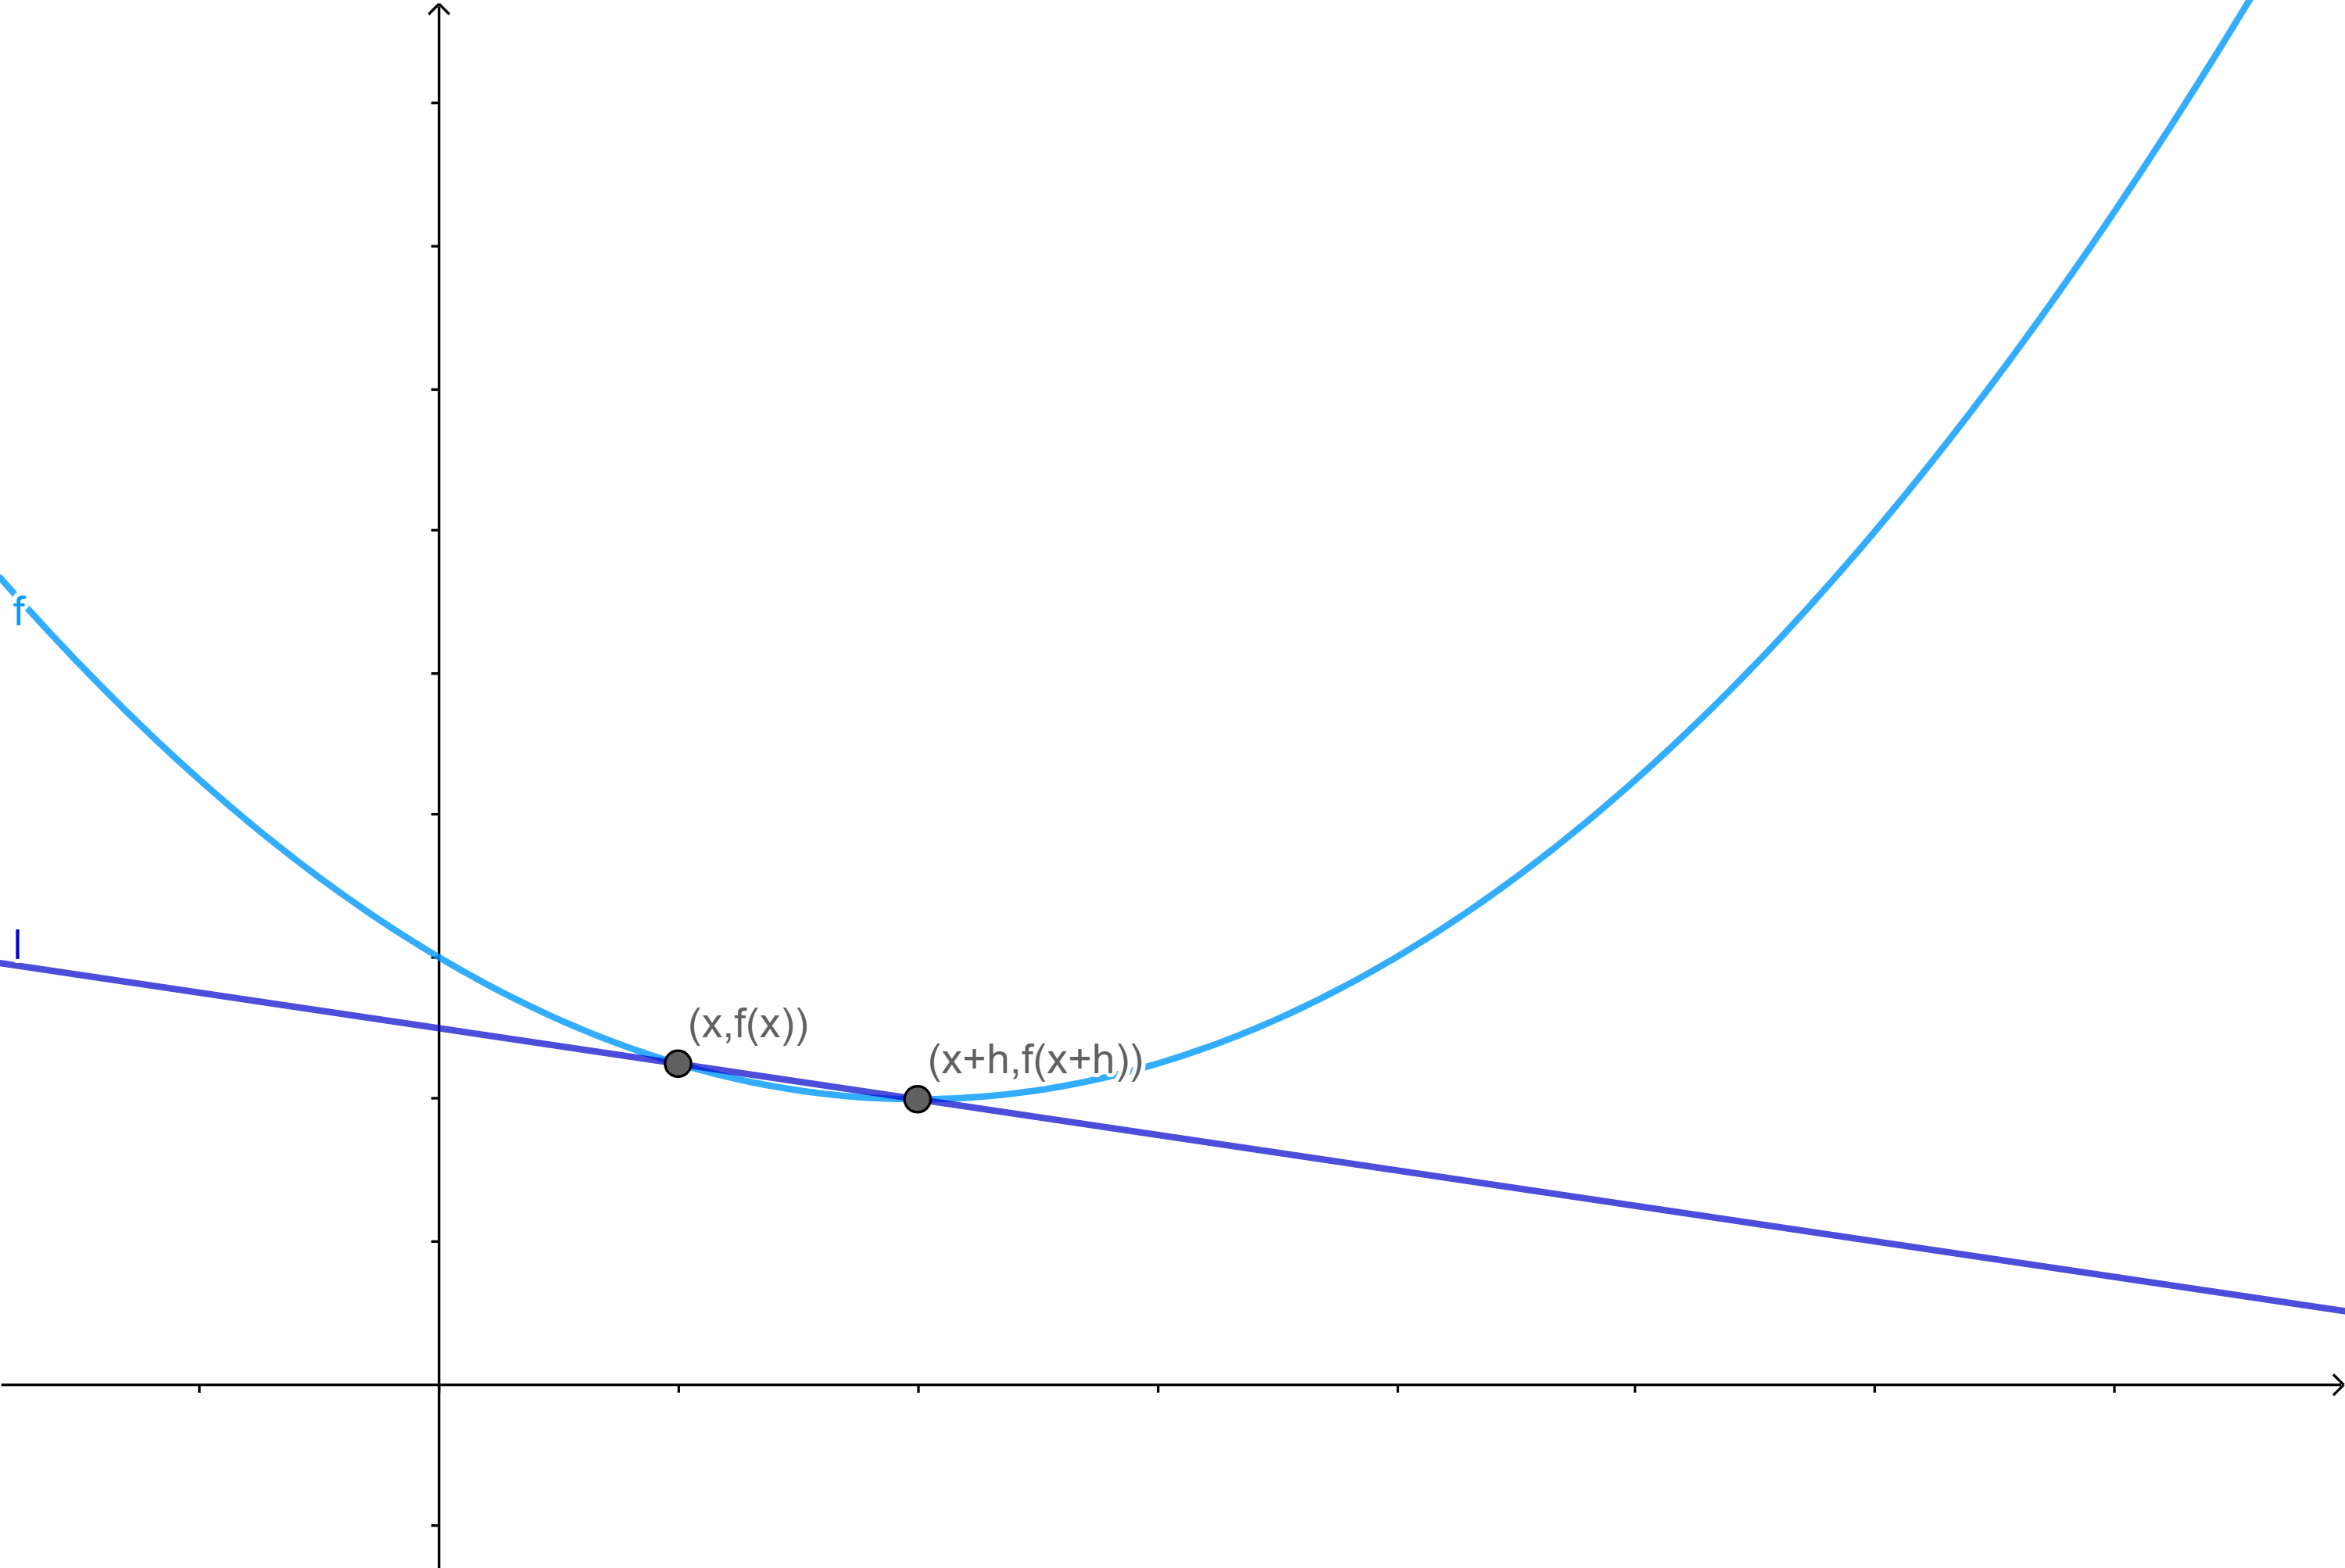
\includegraphics[width = 8cm]{Billeder/sekant2.png}
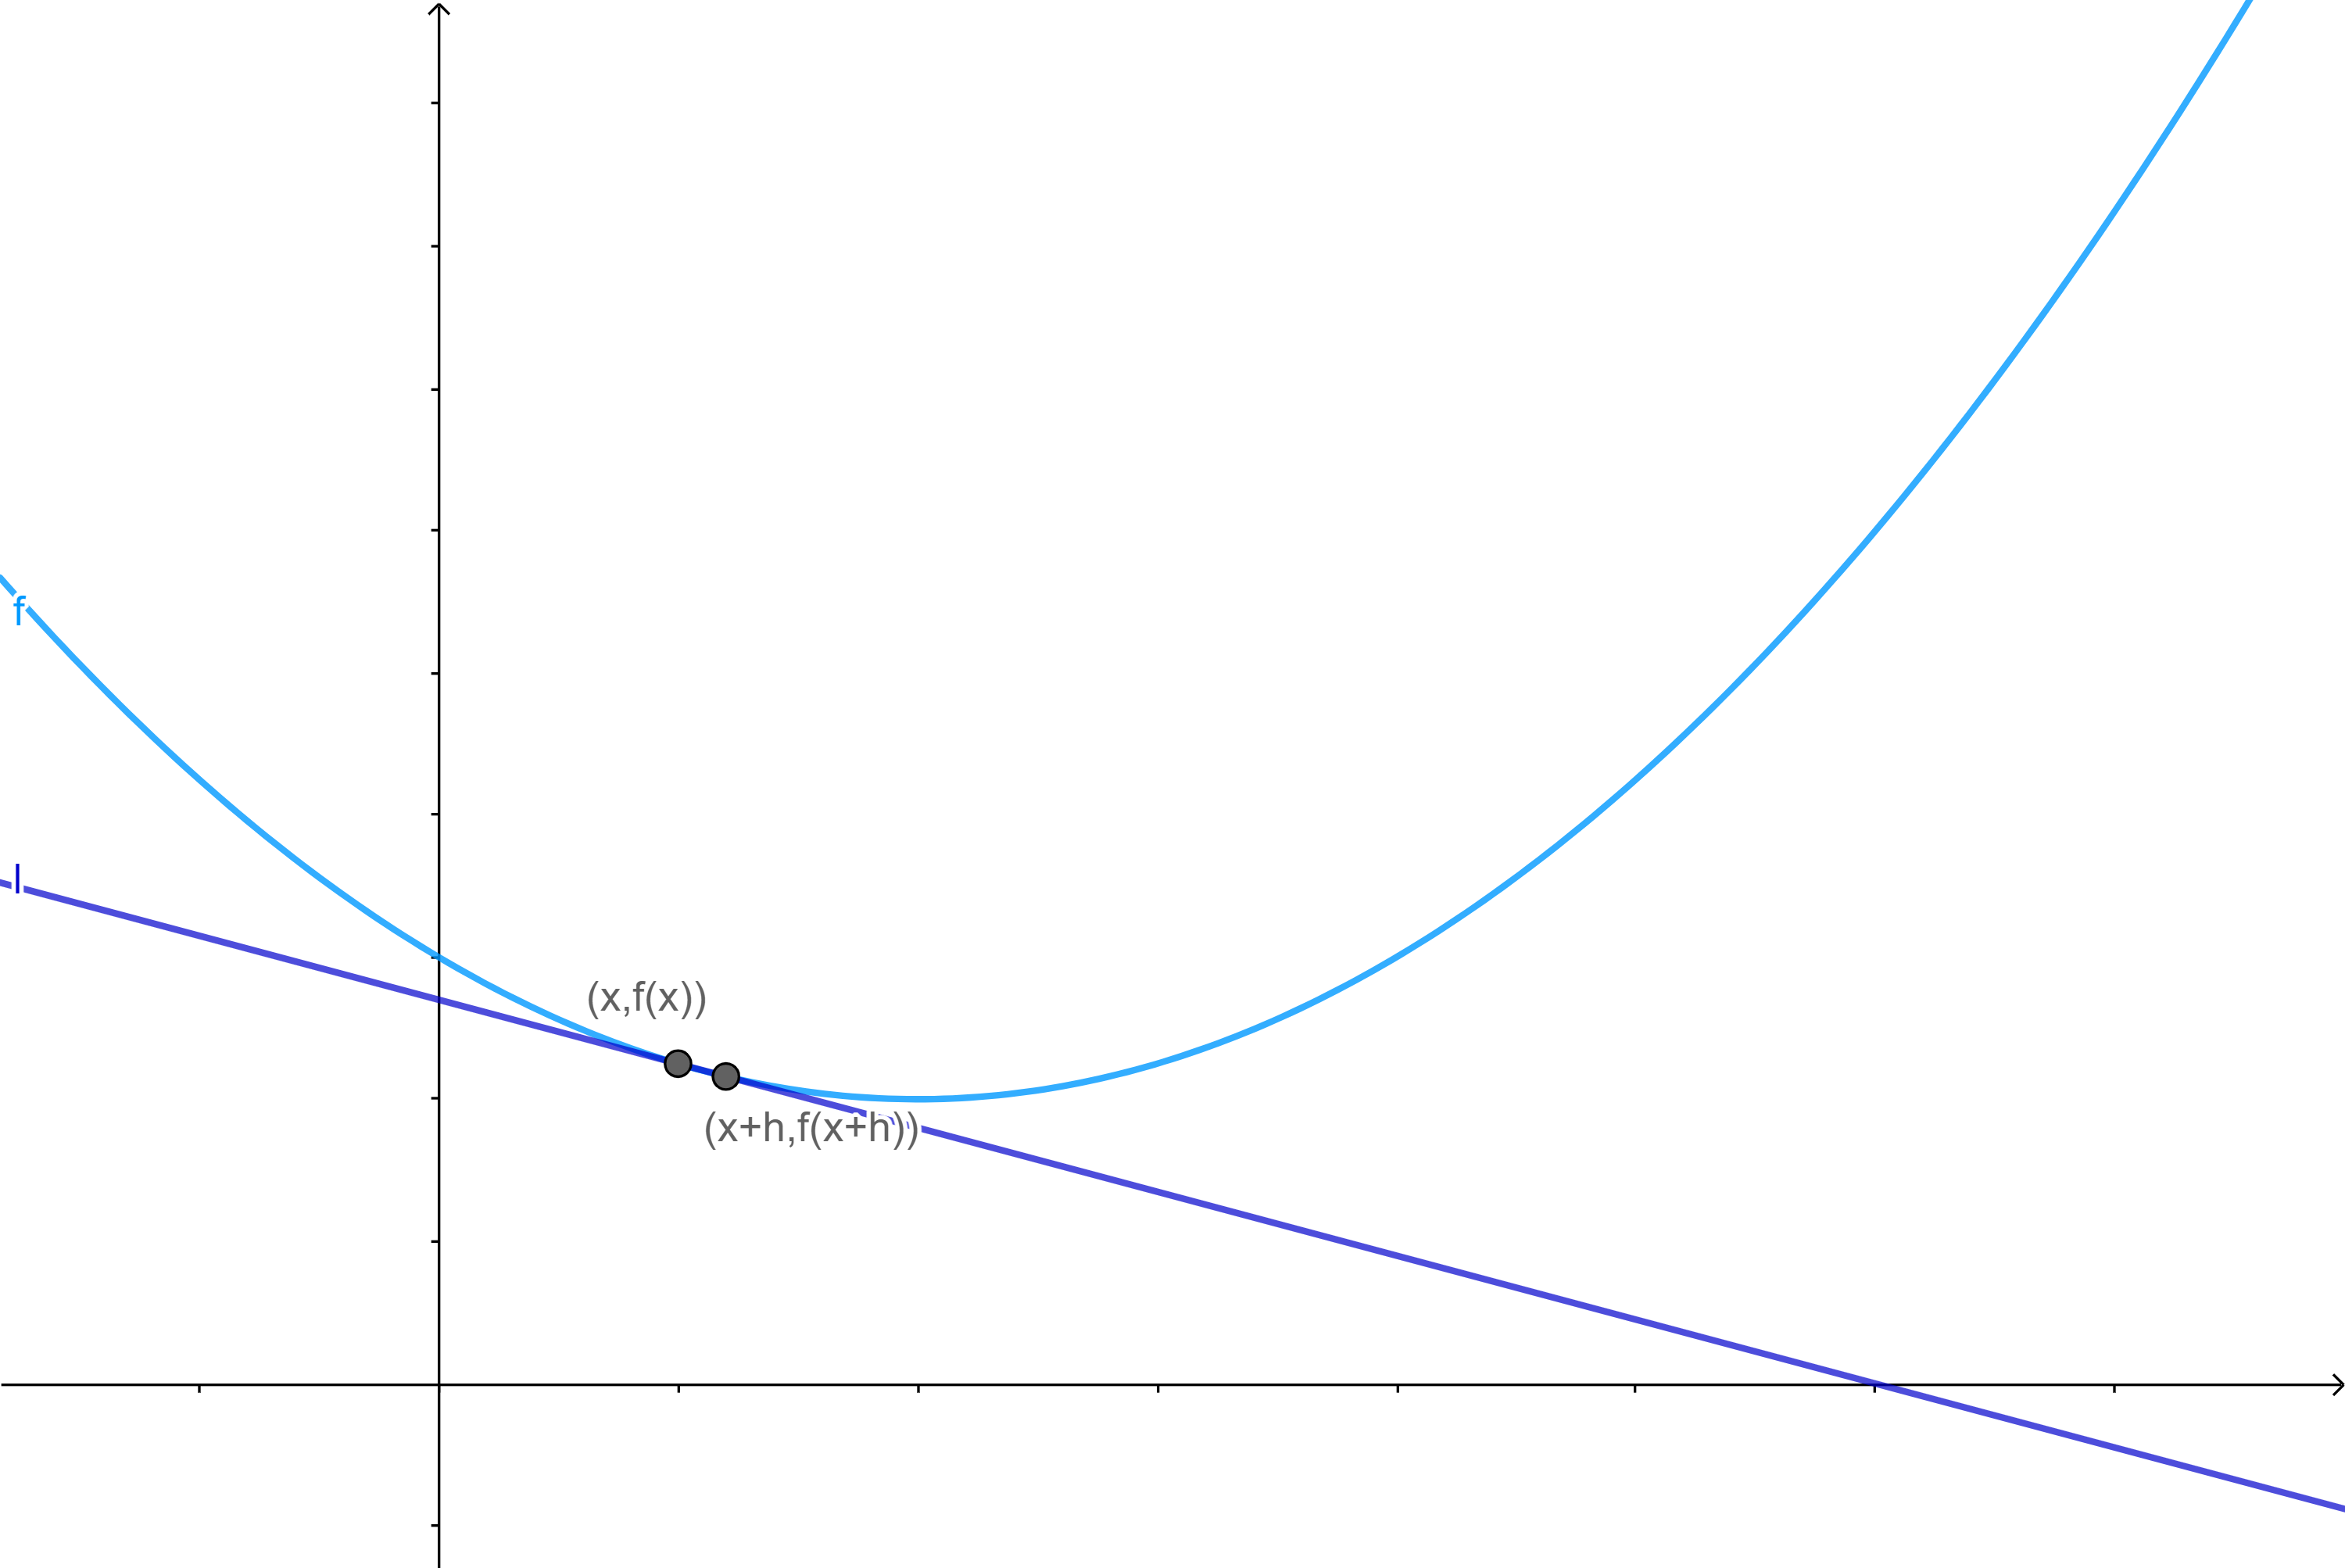
\includegraphics[width = 8cm]{Billeder/sekant3.png}
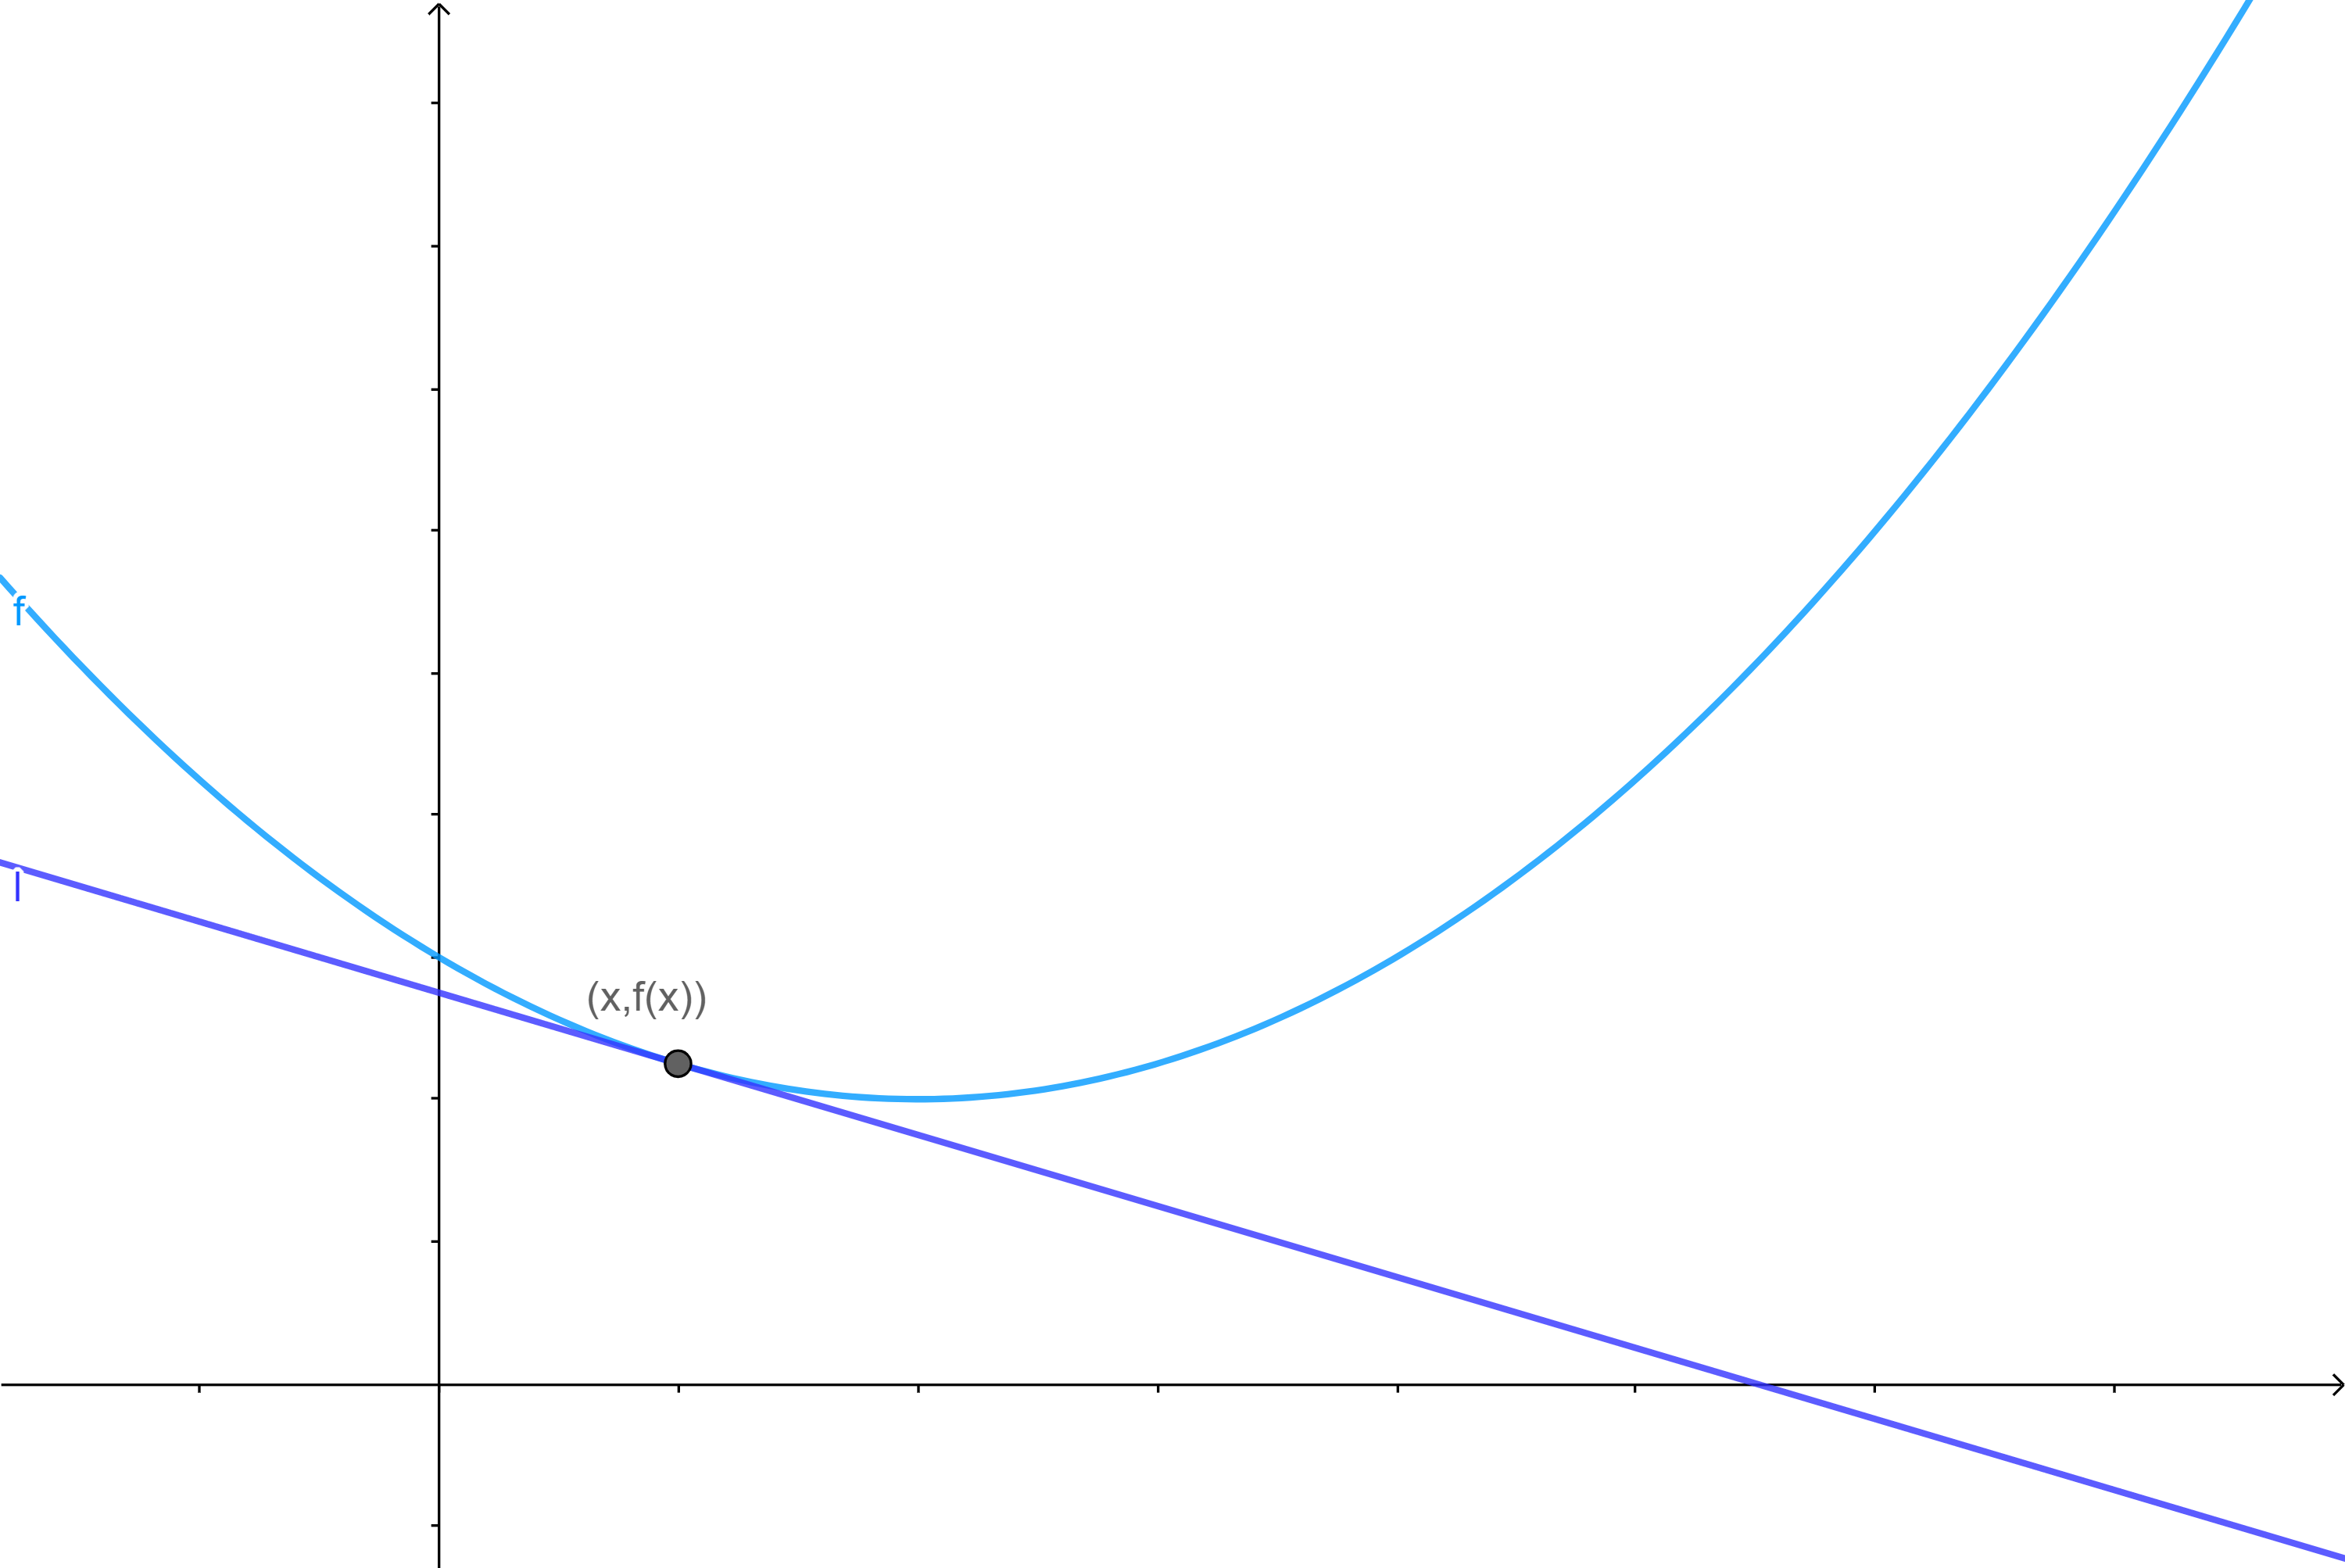
\includegraphics[width=8cm]{Billeder/tangent1.png}
\caption{Sekanterne gennem punkterne $(x,f(x))$ og $(x+h,f(x+h))$, når vi mindsker $h$. }
\label{fig:sek2}
\end{figure}
Det er hældningen af tangenten, vi har interesse i. Hældningen af sekanterne fra Fig. \ref{fig:sek1} og Fig. \ref{fig:sek2} er givet ved
\begin{align*}
\frac{f(x+h)-f(x)}{x+h-x} = \frac{f(x+h)-f(x)}{h}.
\end{align*}
Denne kaldes for differenskvotienten. Vi vil bestemme grænseværdien af differenskvotienten, når $h$ går mod $0$. Dette betegner vi med $\lim_{h\to 0}$, hvilket leder os til følgende definition:
\begin{defn}
Hvis grænsen 
\begin{align*}
\lim_{h\to 0} \frac{f(x+h)-f(x)}{h}
\end{align*}
eksisterer, så siger vi, at funktionen $f$ er differentiabel i $x$. Ydermere, så kalder vi grænseværdien 
\begin{align*}
f'(x) = \lim_{h\to 0} \frac{f(x+h)-f(x)}{h}
\end{align*}
for differentialkvotienten af $f$ i punktet $x$. 
\end{defn}
Vi vil ikke komme mere ind på, hvad det specifikt betyder, at en grænseværdi eksisterer, men løst sagt går det ud på, at grænsen går mod et bestemt tal og ikke divergerer. 
differentialkvotienten kaldes også for den afledede af $f$ eller $f$-mærke. 
\section*{Differentiation af udvalgte funktioner}.
\stepcounter{section}
Vi vil se på en række regneregler for differentiation af kendte funktioner. 
\begin{setn}
Vi har følgende sammenhæng mellem funktioner $f$ og afledede funktion $f'$.
\begin{center}
\begin{tabular}{c|c}
$f(x)$& $f'(x)$\\
\hline
\textnormal{konstant}&$0$\\
\hline
x&$1$\\
\hline
$ax+b$&$a$\\
\hline
$x^2$&$2x$\\
\hline
$x^3$&$3x^2$\\
\hline
$\frac{1}{x}$&$-\frac{1}{x^2}$\\
\hline
$\sqrt{x}$&$\frac{1}{2\sqrt{x}}$
\end{tabular}
\end{center}
\end{setn}
Vi har også mere generelle regneregler.
\begin{setn}
Lad $f$ og $g$ være differentiable i $x$, og lad $k$ være en konstant. Så er funktionerne
\begin{align*}
&f(x) + k,\\
&kf(x),\\
&f(x)+g(x) \textnormal{ og}\\
&f(x)-g(x)
\end{align*}
differentiable. De har følgende differentialkvotienter:
\begin{align*}
(f(x)+k)'&= f'(x),\\
(kf(x))' &= kf'(x),\\
(f(x)+g(x))' &= f'(x)+g'(x),\\
(f(x)-g(x))' &= f'(g)-g'(x).
\end{align*}
\end{setn}
Vi vil senere se beviser for disse sætninger. 
\begin{exa}
Vi ønsker at differentiere funktionen $f(x) = 3x^2-\sqrt{x}$. Hvert led differentieres for sig og vi får
\begin{align*}
f'(x) = (3x^2)' -(\sqrt{x})' = 3(x^2)' - (\sqrt{x})' = 3\cdot 2x - \frac{1}{2\sqrt{x}}.
\end{align*}
\section*{Opgave 1}
Bestem den afledede funktion til følgende funktioner:
\begin{align*}
&1) \ x^3+2x  &&2) \  2\sqrt{x}+10  \\
&3) \ 2x+4  &&4) \ x^3+x^2+x+1   \\
&5) \ 7-10\sqrt{x}+7x^3 &&6) \ 4x^3-12\sqrt{x}    \\
&7) \ \frac{1}{x} + \frac{x^2}{5} -2x +1 &&8) \  \frac{2x^3}{3}-\frac{4}{x}   \\
&9) \ \sqrt{x}+\sqrt{2}  &&10) \  \frac{\sqrt{2}}{2}+x^3-\frac{11\sqrt{x}}{5}  \\
\end{align*}
\section*{Opgave 2}
Bestem hældningen af tangenterne punkterne $(1,f(1))$ og $ (2,f(2))$ af følgende funktioner:
\begin{align*}
&1) \ 5x^2+10   &&2) \ \sqrt{x}    \\
&3) \ \frac{\sqrt{x}}{3} + x^3  &&4) \ \frac{2}{x}   \\
&5) \ 7   &&6) \ \frac{7\sqrt{x}}{2} + \frac{1}{x}   \\
&7) \ x^2+x^3+1  &&8) \ \frac{1}{3}x^3+\frac{1}{2}x^2 + x    \\
&9) \ \frac{10}{3} + x+3\sqrt{x}   &&10) \ 7+\frac{1}{3} + x^3 + \frac{2}{x}    \\
\end{align*} 
\end{exa}